%\title{EMC LaTeX Portrait Poster Template}
%%%%%%%%%%%%%%%%%%%%%%%%%%%%%%%%%%%%%%%%%
% a1poster Portrait Poster
% LaTeX Template
% Version 2.0 (22/06/16)
%
% The a1poster class was created by:
% Joe Rowing (JoeRowing@exeterms.ac.uk)
% 
% This template has been produced by:
% Joe Rowing at Exeter Mathematics School
%
% License:
% CC BY-NC-SA 3.0 (http://creativecommons.org/licenses/by-nc-sa/3.0/)
%
%%%%%%%%%%%%%%%%%%%%%%%%%%%%%%%%%%%%%%%%%

%----------------------------------------------------------------------------------------
%   PACKAGES AND OTHER DOCUMENT CONFIGURATIONS
%----------------------------------------------------------------------------------------

\documentclass[a1,portrait]{a1poster}

\usepackage{multicol} % This is so we can have multiple columns of text side-by-side
\columnsep=50pt % This is the amount of white space between the columns in the poster
\columnseprule=0.01pt % This is the thickness of the black line between the columns in the poster

\usepackage[svgnames]{xcolor} % Specify colors by their 'svgnames', for a full list of all colors available see here: http://www.latextemplates.com/svgnames-colors

\usepackage{times} % Use the times font


\usepackage{graphicx} % Required for including images
\graphicspath{{figs/}} % Location of the graphics files
\usepackage{booktabs} % Top and bottom rules for table
\usepackage[font=small,labelfont=bf]{caption} % Required for specifying captions to tables and figures
\usepackage{amsfonts, amsmath, amsthm, amssymb} % For math fonts, symbols and environments
\usepackage{wrapfig} % Allows wrapping text around tables and figures
\usepackage{hyperref}
\usepackage[epsilon, tsrm, altpo]{backnaur}
\usepackage{listings}
\usepackage{paracol}
\lstset{language=Haskell, upquote=true, stringstyle=\ttfamily, showstringspaces=true}

% https://tex.stackexchange.com/questions/450226/how-to-avoid-column-vertical-line-inside-multicol-environment
\setlength{\columnseprule}{0pt}

\begin{document}

%----------------------------------------------------------------------------------------
%   POSTER HEADER 
% The header is divided into two boxes:
% The first is 75% wide and houses the title, subtitle, names, university/organization and contact information
% The second is 25% wide and houses the EMS Logo
% 
%----------------------------------------------------------------------------------------

\begin{minipage}[b]{0.6\linewidth}
\huge \color{DarkRed} \textbf{Quick and Reusable Code Generation for Idris} \color{Black}\\ % Title
\huge\textit{Integrating dependent types into the industrial services}\\[1cm] % Subtitle
\large \textbf{Taine Zhao \& Yukiyoshi Kameyama}\\[0.5cm] % Author(s)
\large Computer Science, University of Tsukuba \\[0.2cm] % University/organization
\texttt{thaut@logic.cs.tsukuba.ac.jp; kam@cs.tsukuba.ac.jp}\\
\end{minipage}
%
% \begin{minipage}[b]{0.4\linewidth}
% 
\includegraphics[width=15cm]{emsnew.PNG}\\
% \end{minipage}

\vspace{.5cm} % A bit of extra whitespace between the header and poster content

%----------------------------------------------------------------------------------------

\begin{multicols}{2} % This is how many columns your poster will be broken into, by convention a portrait poster is generally split into 2 or 3 columns

%----------------------------------------------------------------------------------------
%   ABSTRACT

%An abstract is a brief summary of a research article, thesis, review, conference proceeding or any in-depth analysis of a particular subject and is often used to help the reader quickly ascertain the paper's purpose
%----------------------------------------------------------------------------------------

% \color{CornflowerBlue} % Colour for the abstract

\section*{Abstract}

As a dependently-typed functional programming languages, Idris shows
quite a high expressiveness with its type system under a considerably strong static guarantee.

To leverage these powerful static programming language features for
existing industrial applications safer and more expressive,
we're supposed to implement code generation back ends for Idris.

Whereas Idris has already provided convenient interfaces to support
agnostic back ends, it is still cumbersome to import Idris programs
into an existing programming language, as the latter is already
in a large amount and continuously proliferating, and the implementations
of each back end certainly have quite a few overlaps.
  
To address this, we introduce a "common" intermediate representation
powered by Tagless Final Style, which contributes to the reuse most of the tasks
required by an Idris back end. As a result, we allow making a Idris back end
in a most simplified routine, which can usually be accomplished in few hours
or even minutes.

%----------------------------------------------------------------------------------------
%   INTRODUCTION

%Avoid using technical definitions unless absolutely necessary. The introduction section is here to introduce your issue, so be sure to not bore your readers right away with excessive information. You can even include graphics if they will help the viewer understand the work that you have done.
%----------------------------------------------------------------------------------------

% \color{OrangeRed} % color for the introduction

\section*{Background}

% \includegraphics[width=15cm]{Idris-Backend-For-Free.png}\\
Idris has already made lots of efforts to their code generation, where
they provided various IRs \cite{brady2015cross} to start a custom back end.

We provide a concise version of their defunctionalised IR with some details omitted, hereafter as $DDecl$.

\vspace{-1cm}

\begin{multicols}{2}

\begin{minipage}[b]{0.8\linewidth}
\begin{bnf*}
    \bnfprod{expr}{\bnftd{Var} \bnfsp \bnftd{name}}\\
    \bnfmore{\bnfor \bnftd{App} \bnfsp \bnftd{bool} \bnfsp \bnftd{name} \bnfsp \bnftd{expr}}\\
    \bnfmore{\bnfor \bnftd{Let} \bnfsp \bnftd{name} \bnfsp \bnftd{expr} \bnfsp \bnftd{expr}}\\
    \bnfmore{\bnfor \bnftd{Update} \bnfsp \bnftd{name} \bnfsp \bnftd{expr}}\\
    \bnfmore{\bnfor \bnftd{Proj} \bnfsp \bnftd{expr} \bnfsp \bnftd{int}}\\
    \bnfmore{\bnfor \bnftd{Cons} \bnfsp \bnftd{name} \bnfsp \bnfts{[} \bnftd{expr}\bnfts{]}}\\
    \bnfmore{\bnfor \bnftd{Case} \bnfsp \bnftd{expr} \bnfsp \bnfts{[} \bnfpn{alt}\bnfts{]}}\\
    \bnfmore{\bnfor \bnftd{Const} \bnfsp \bnftd{constant-literal}}\\
    \bnfmore{\bnfor \bnftd{Foreign} \bnfsp \bnftd{fdesc} \bnfsp \bnftd{fdesc} \bnfsp \bnfts{[} \bnftd{(} \bnfsp \bnftd{fdesc} \bnfsp \bnftd{,} \bnfsp \bnftd{expr} \bnfsp \bnftd{)}\bnfts{]}}\\
    \bnfmore{\bnfor \bnftd{Op} \bnfsp \bnftd{primitive-op} \bnfsp \bnfts{[} \bnftd{expr}\bnfts{]}}\\
    \bnfmore{\bnfor \bnftd{DoNothing}}\\
    \bnfmore{\bnfor \bnftd{Error} \bnfsp \bnftd{string}}\\
\end{bnf*}
\end{minipage}

\begin{minipage}[b]{1\linewidth}
\begin{bnf*}
    \bnfprod{alt}{\bnftd{ConCase} \bnfsp \bnftd{name} \bnfsp \bnfts{[} \bnftd{name}\bnfts{]} \bnfsp \bnftd{expr}}\\
    \bnfmore{\bnfor \bnftd{ConstCase} \bnfsp \bnftd{constant-literal} \bnfsp \bnftd{expr}}\\
    \bnfmore{\bnfor \bnftd{DefaultCase} \bnfsp \bnftd{expr}}\\
    \bnfprod{decl}{\bnftd{DefFun} \bnfsp \bnftd{name} \bnfsp \bnfts{[} \bnftd{name}\bnfts{]} \bnfsp \bnftd{expr}}\\
    \bnfmore{\bnfor \bnftd{DefCons} \bnfsp \bnftd{name} \bnfsp \bnftd{int}}\\   
    \bnfprod{arith-type}{\bnftd{float} \bnfor \bnftd{int}}\\
    \bnfprod{primitive-op}{\bnftd{sdiv} \bnfsp \bnftd{arith-type}}\\
    \bnfmore{\bnfor \bnftd{udiv} \bnfsp \bnftd{arith-type}}\\
    \bnfmore{\bnfor \bnftd{+} \bnfsp \bnftd{arith-type}}\\
    \bnfmore{\bnfor \bnftd{-} \bnfsp \bnftd{arith-type}}\\
    \bnfmore{\bnfor \bnftd{*} \bnfsp \bnftd{arith-type}}\\
    \bnfmore{\bnfor \bnftd{...}}
\end{bnf*}
\end{minipage}
\end{multicols}

\vspace{-0.5cm}

\begin{itemize}
    \setlength\itemsep{-0.2em}
    \item $Cons$, $DefCons$ : constructing tagged unions, and constructor definitions
    \item $Case$ : pattern matching, or deconstructions
    \item $Proj$ : projections, on tuples and tagged unions
    \item $primitive-op$ : $+$, $-$, $*$, $/$, and other primitive operators defined and used by Idris compiler

\end{itemize}

This IR is already convenient, however still cannot we gain code reuse or avoid repetitions,
when implementing distinct back ends.

Firstly we check $Let$ expressions. They are responsible for variable introductions,
and also capable of \textbf{shadowing variables}, but unfortunately missing in most old programming languages
such as C/C++, Java, Ruby, Python, etc.

\begin{multicols}{3}

\begin{minipage}[b]{1\linewidth}
\begin{center}\vspace{0.1cm}
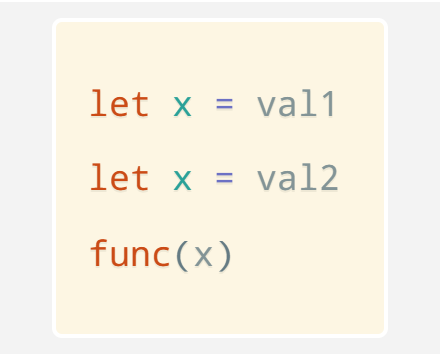
\includegraphics[width=0.9\linewidth]{figs/let.png}
\captionof{figure}{\color{DarkRed} $let$ in $DDecl$}
\end{center}\vspace{0.1cm}
\end{minipage}

\begin{minipage}[b]{1\linewidth}
\begin{center}\vspace{0.1cm}
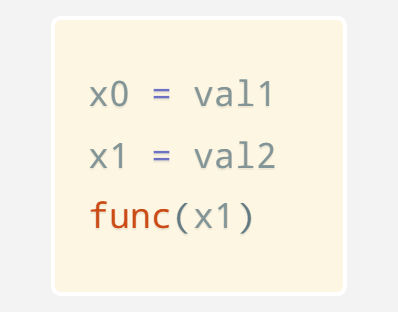
\includegraphics[width=0.9\linewidth]{figs/let-by-mangling.png}
\captionof{figure}{\color{DarkRed} Eliminating $let$ by name mangling}
\end{center}\vspace{0.1cm}
\end{minipage}


\begin{minipage}[b]{1\linewidth}
\begin{center}\vspace{0.1cm}
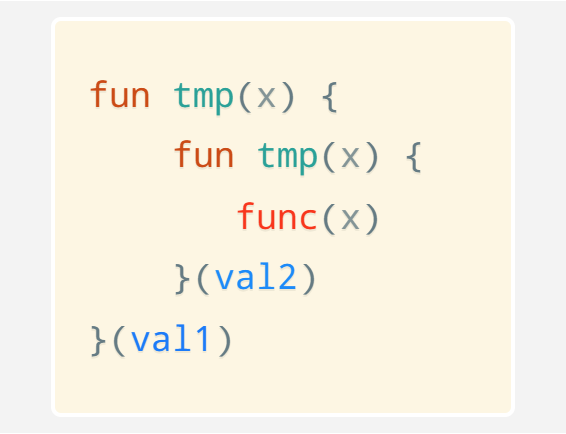
\includegraphics[width=0.9\linewidth]{figs/let-by-im-call.png}
\captionof{figure}{\color{DarkRed} Eliminating $let$ by immediately invoked functions(abbr. IIFE)}
\end{center}\vspace{0.1cm}
\end{minipage}

\end{multicols}

 Eliminating $let$ by IIFE is very handy without requiring much code, however
 extremely \textbf{SLOW} down the back ends of dynamic programming languages.

 As for name mangling,

\begin{itemize}
    \setlength\itemsep{-0.2em}
    \item renaming variables itself needs a simple pass to analyse the scope of your program!
    \item considering register allocation problems?
\end{itemize}

\begin{multicols}{2}

\begin{minipage}[b]{1\linewidth}
\begin{center}\vspace{0.1cm}
    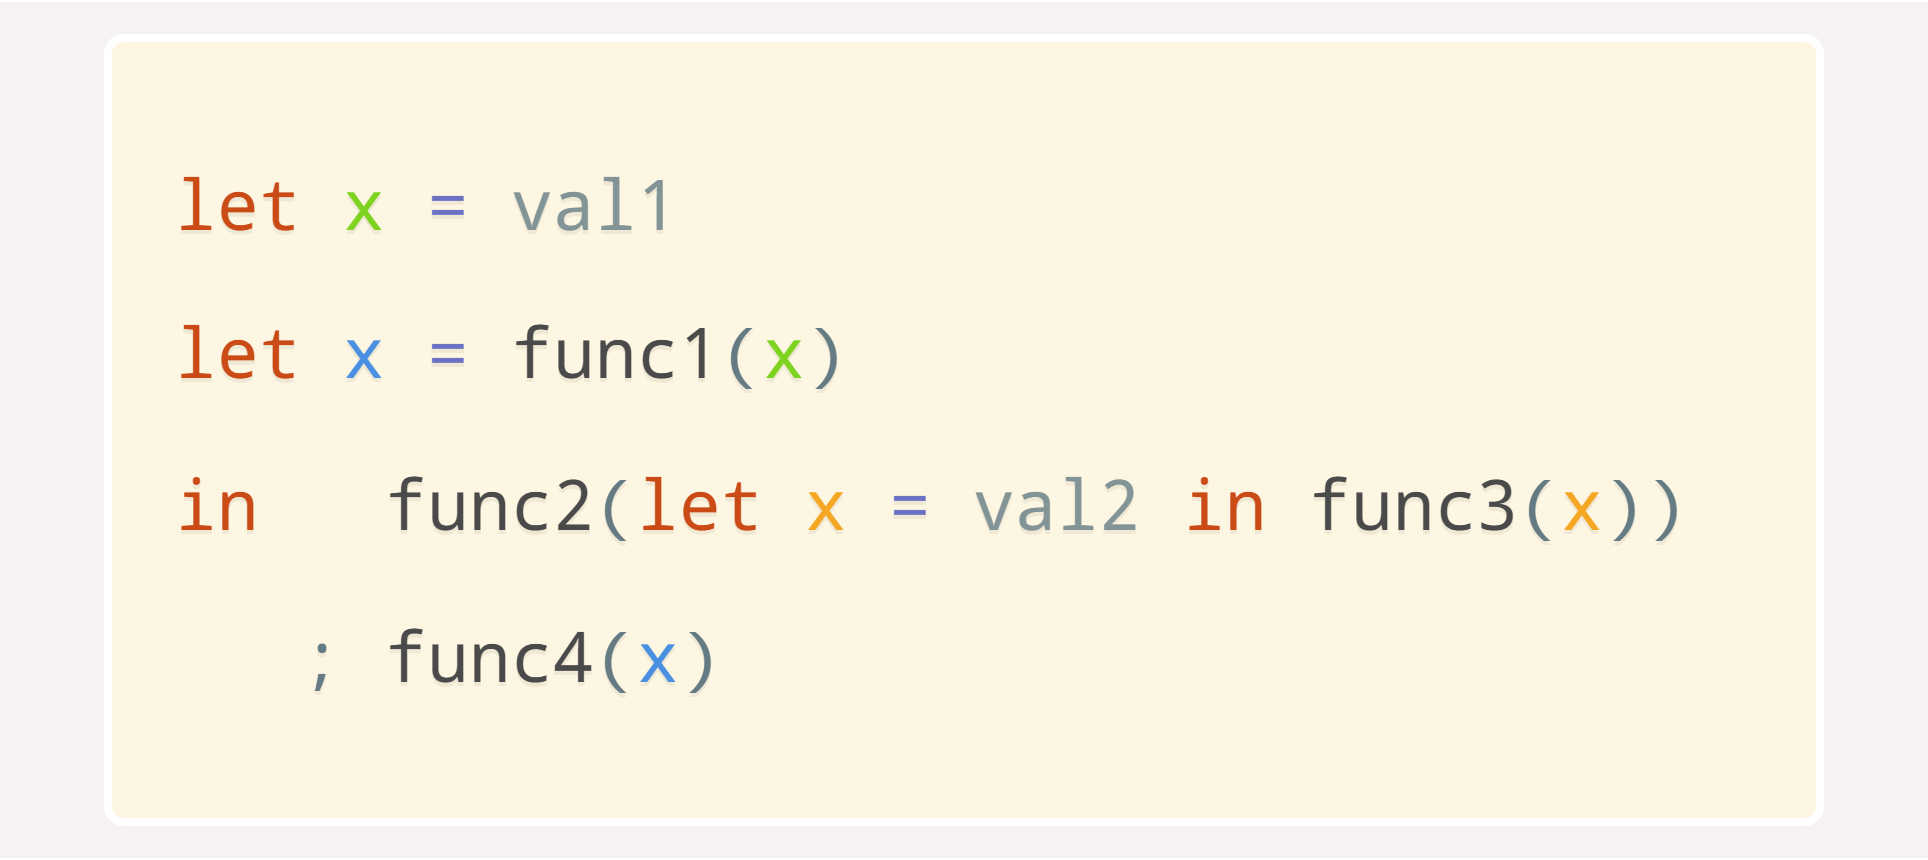
\includegraphics[width=0.9\linewidth]{figs/let-occur.png}
    \captionof{figure}{\color{DarkRed} Occurrences of distinct $x$}
\end{center}\vspace{0.1cm}
\end{minipage}

\begin{minipage}[b]{1\linewidth}
\begin{center}\vspace{0.1cm}
    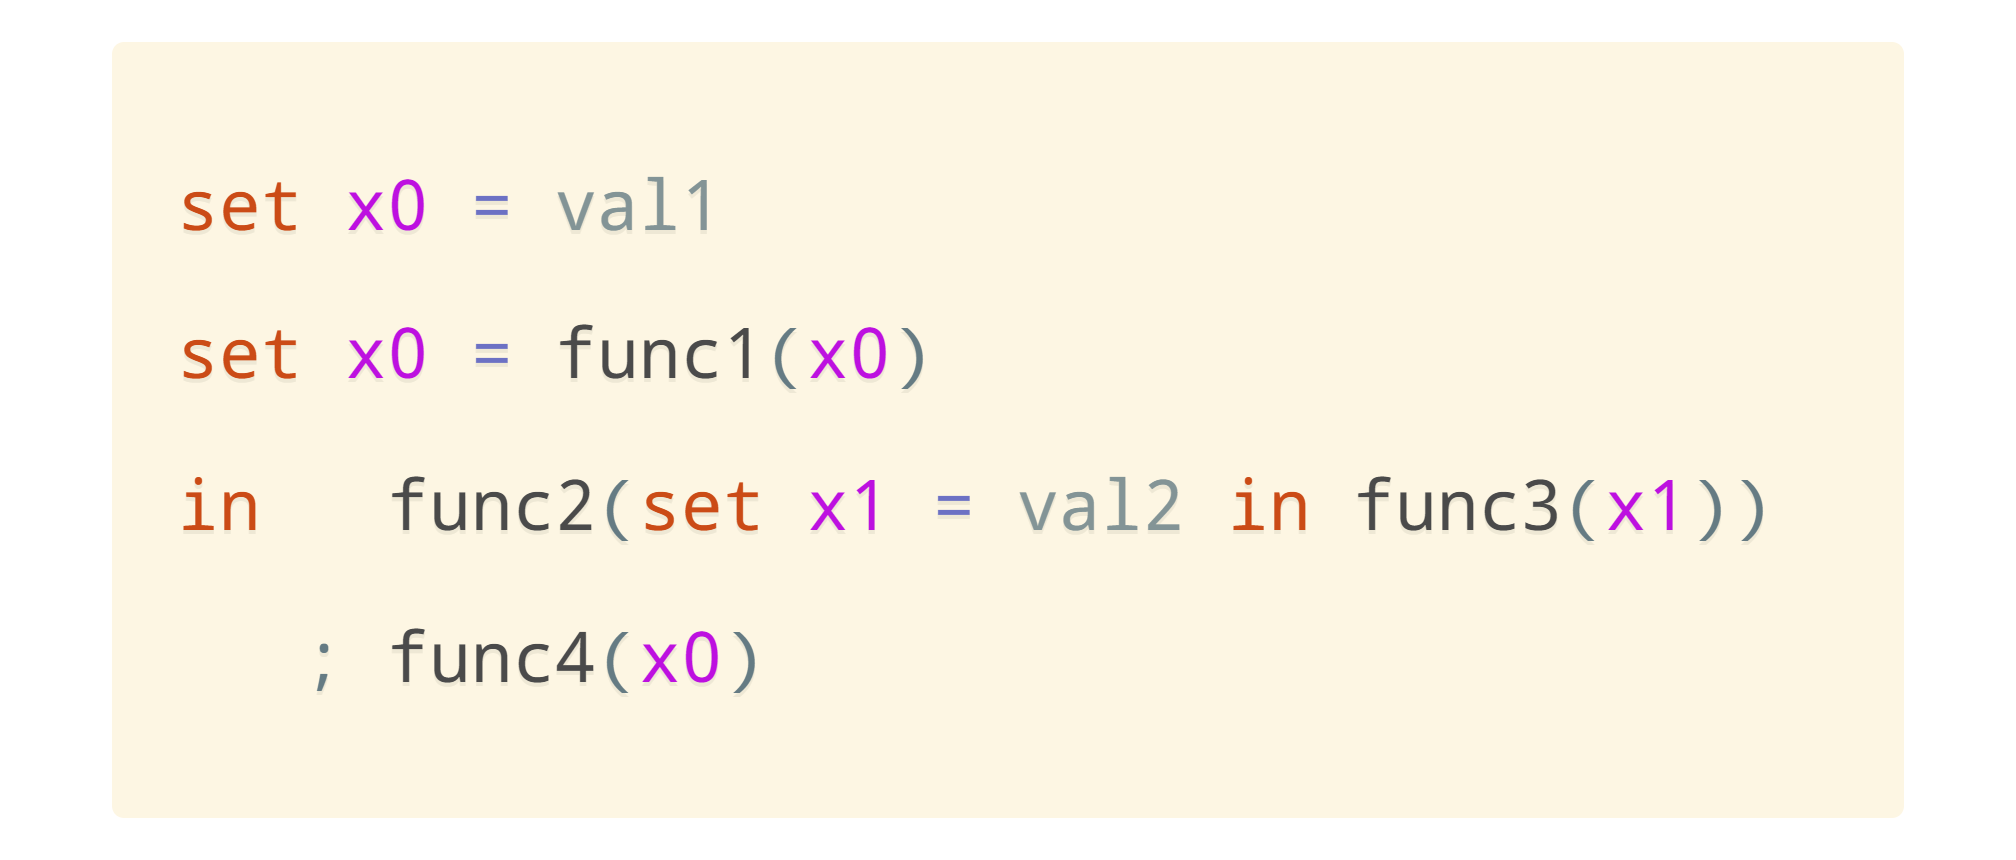
\includegraphics[width=0.9\linewidth]{figs/let-realloc.png}
    \captionof{figure}{\color{DarkRed} Register allocation optimisation for $x$}
\end{center}\vspace{0.1cm}
\end{minipage}
\end{multicols}

Besides, the underlying of ADTs is the representation of the tagged unions.

A valid approach is, firstly emulate LISP symbols to achieve $O(1)$ comparable \textbf{tags},
and then use tuples whose 1st element is a LISP symbol, to represent ADTs.
\begin{multicols}{2}

\begin{minipage}[b]{1\linewidth}
\begin{center}\vspace{0.1cm}
    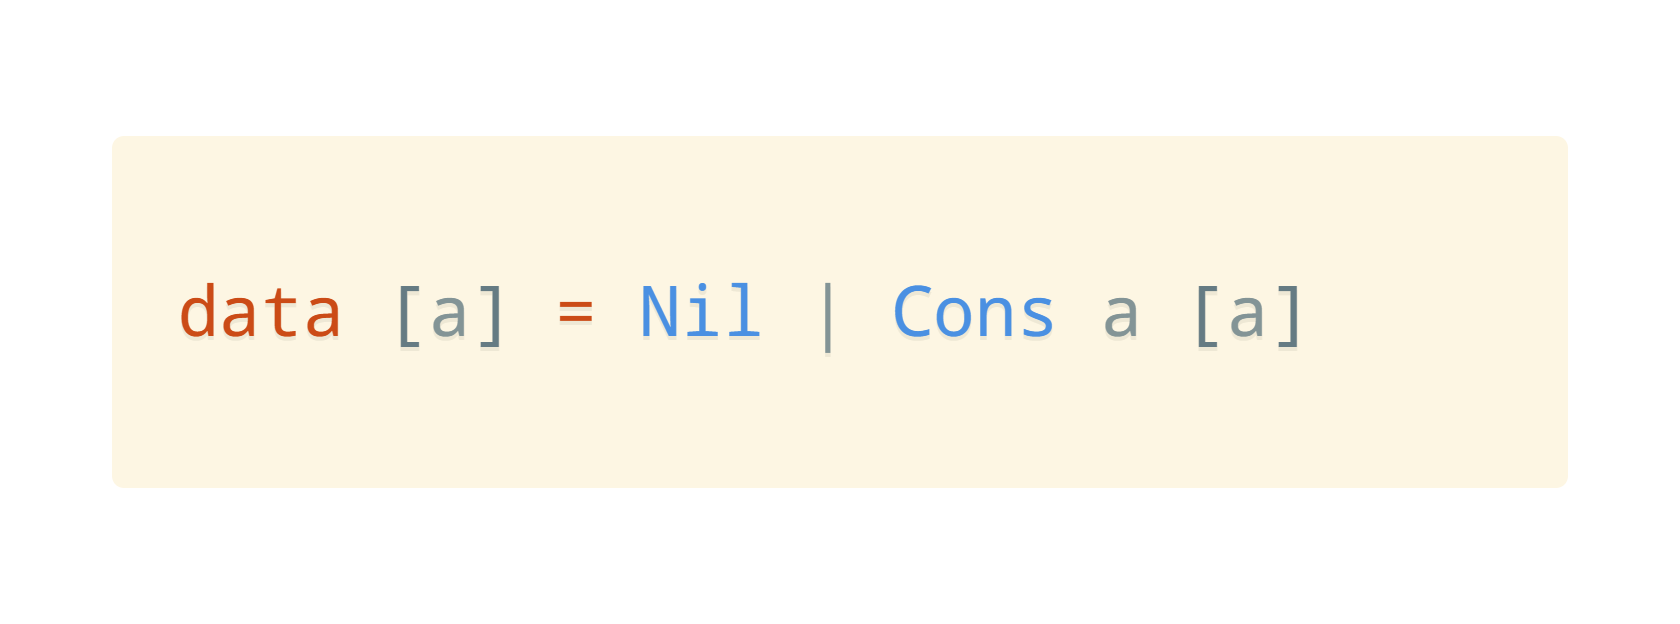
\includegraphics[width=0.9\linewidth]{figs/tagged-union.png}
    \captionof{figure}{\color{DarkRed} Algebraic Data Types(ADTs)}
\end{center}\vspace{0.1cm}
\end{minipage}

\begin{minipage}[b]{1\linewidth}
\begin{center}\vspace{0.1cm}
    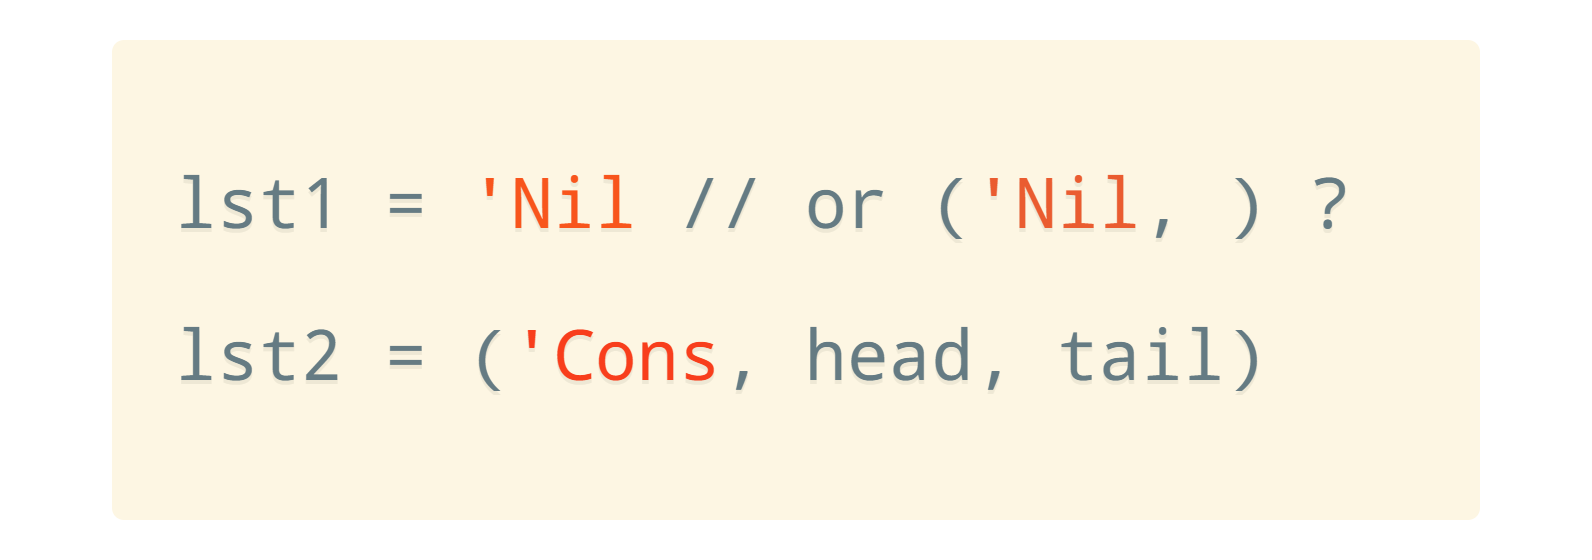
\includegraphics[width=0.9\linewidth]{figs/tagged-union-impl.png}
    \captionof{figure}{\color{DarkRed} ADT internals in back ends}
\end{center}\vspace{0.1cm}
\end{minipage}

\end{multicols}

We also have to

\begin{itemize}
    \setlength\itemsep{-0.1em}
    \item translate pattern matching things to non-pattern match languages
    \item translate block expressions \cite{gcc-stmt-expr} \cite{pep572} into languages whose expressions cannot accommodate statements
    \item support primitive operations
    \item support FFI
\end{itemize}

Options shall be provided here to control the properties of the IR, to achieve the reuse of
\begin{itemize}
    \setlength\itemsep{-0.2em}
    \item desugaring block expressions, which may requires register allocation optimisations.
    \item  desugaring pattern matching to switch statements and if statements
    \item  desugaring data constructors to normal functions
    \item  using LISP-style $Symbol$ as the tag of tagged union, for a language with $Symbol$ data.
    \item  emulation of $Symbol$ in the language without $Symbol$ data for tags of tagged unions
\end{itemize}

Those stuffs are not difficult, but quite annoying when implementing
them again and again, for each back end.

What is the possibly simplest IR for code generation?

\section*{Proposal}

To address problems mentioned above, We hereby propose an IR,
which is lightweight, neat and compact, and finally capable of
getting used to support a back end quickly.

\vspace{-1.5cm}
\begin{multicols}{2}

\begin{minipage}[t]{0.8\linewidth}
\begin{bnf*}
    \bnfprod{block-stmt}{\bnfts{[} \bnftd{stmt} \bnfts{]}}\\
    \bnfprod{stmt}{\bnftd{Update} \bnfsp \bnftd{name} \bnfsp \bnftd{expr}}\\
    \bnfmore{\bnfor \bnftd{DefFun} \bnfsp \bnftd{name} \bnfsp \bnfts{[} \bnftd{name}\bnfts{]} \bnfsp \bnftd{block-stmt}}\\
    \bnfmore{\bnfor \bnftd{Switch} \bnfsp \bnftd{expr} \bnfsp \bnfts{[} \bnfts{(} \bnfsp \bnftd{constant-literal} \bnfsp \bnftd{,} \bnfsp \bnftd{block-stmt} \bnfsp \bnfts{)}\bnfts{]}}\\
    \bnfmore{\bnfor \bnftd{If} \bnfsp \bnftd{expr} \bnfsp \bnftd{block-stmt} \bnfsp \bnftd{block-stmt}}\\
\end{bnf*}
\end{minipage}

\vfill\null
\columnbreak

\begin{minipage}[t]{0.8\linewidth}
\begin{bnf*}
    \bnfprod{lvar}{\bnftd{name} \bnfor \bnftd{constant-literal}}\\
    \bnfprod{expr}{\bnftd{Var} \bnfsp \bnftd{name}}\\
    \bnfmore{\bnfor \bnftd{App} \bnfsp \bnftd{name} \bnfsp \bnfts{[} \bnftd{lvar} \bnfts{]}}\\
    \bnfmore{\bnfor \bnftd{Const} \bnfsp \bnftd{constant-literal}}\\
\end{bnf*}
\end{minipage}
\end{multicols}
\captionof{figure}{\color{DarkRed} Weakest Declarations}

Instead of leaving a blank for the internal implementations of tuples, FFIs, constructors of algebraic data,
we can assume a generally applicable implementation, and transform $DDecl$ to the proposed IR, which we'd call
it a \textbf{Weakest Declaration}(abbr. $WDecl$).


$WDecl$ desugars $Let$ expressions to $Update$ statements, simplifies function arguments to accept variables or constants only,
and avoids requirement of expressing block expressions in the target language.

Further, we point out some correspondences between the original $DDecl$ and our $WDecl$.

%


% \begin{center}
% \begin{table}
% \begin{tabular}{ |c|c|c| } 
% \hline
% \textbf{Cases} & \textbf{DDecl} & \textbf{WDecl}                                   \\ \hline
% Addition Integers & \lstinline!Op (+ int) a b!  & \lstinline!App "+" [int, a, b])! \\ \hline
% Projections & \lstinline!Proj a 1! & \lstinline!App "proj" [a, 1]!                 \\ \hline
% Pattern Matching 1 & \lstinline!Case a [ConstCase 1 233]! & \lstinline!Switch a [(1, 233)]! \\ \hline
% Pattern Matching 2 & \lstinline!Case a [ConCase "Cons" [_, _] 321]! & \lstinline!Switch App "proj" [a, 0] [("Cons", 321)]! \\ \hline
% Pattern Matching 2 & \lstinline!Case a [ConCase "Cons" [_, _] 321]! & \lstinline!Switch App "proj" [a, 0] [("Cons", 321)]! \\ \hline
% Construction 1 & \lstinline!Cons "Nil" []! & \lstinline!App "make_symbol" ["Nil"]! \\ \hline
% Construction 2 & \lstinline!Cons "Cons" [1, a]! & \lstinline!App "make_tuple" [App "make_symbol" ["Cons"], 1, a]! \\ \hline
% \end{tabular}
% \end{table}
% \end{center}
% \captionof{table}{\color{DarkRed} Correspondences between $DDecl$ and $WDecl$}

\begin{center}
\begin{tabular}{ |c|c|c| } 
 \toprule
 \textit{Cases} & \textit{DDecl} & \textit{WDecl} \\
 \midrule
 Addition Integers & \lstinline!Op (+ int) a b!  & \lstinline!App "+" [int, a, b])! \\
 \midrule
 Projections & \lstinline!Proj a 1! & \lstinline!App "proj" [a, 1]!                 \\
 \midrule
 Pattern Matching 1 & \lstinline!Case a [ConstCase 1 233]! & \lstinline!Switch a [(1, 233)]! \\
 \midrule
 Pattern Matching 2 & \lstinline!Case a [ConCase "Cons" [_, _] 321]! & \lstinline!Switch App "proj" [a, 0] [("Cons", 321)]! \\
 \midrule
 Construction 1 & \lstinline!Cons "Nil" []! & \lstinline!App "make_symbol" ["Nil"]! \\
 \midrule
 Construction 2 & \lstinline!Cons "Cons" [1, a]! & \lstinline!App "make_tuple" [App "make_symbol" ["Cons"], 1, a]! \\
 \bottomrule
\end{tabular}
\end{center}

In the above table, for being concise, we omitted the constructions of \lstinline!Const!,
but simply use literals like \lstinline!1!, \lstinline!321!, \lstinline!"+"! instead.



% 2 common ways of eliminating $Let$ expressions are illustrated in above boxes, where
% the approach by immediately invoked function expressions(abbr. IIFE) is straightforward,
% and can be achieved without much code.

% Yet, function calls in dynamic programming languages without JIT compilation can be particularly slow.
% For instance, in Python, addition as a function is about 2.5 slower than addition as a binary operation.

% Other than a performance concern, eliminating $Let$ by IIFE may also produce
% stack overflow errors, because combinations of $Let$ expressions lead to nested function calls,
% unlike a series of parallel assignments.

% Hence, to support back ends of some dynamic programming languages, we shall use name mangling instead of IIFE,
% to achieve a better performance, and get rid of stack overflow.

\color{FireBrick} %  colour for the conclusions to make them stand out

\section*{Results}

We implemented the transformation from $DDecl$ to $WDecl$ in the Haskell side,
produce it a binary executable, which implements the Idris back end interfaces.

Hence, we become capable of compiling an Idris project, fetching its $WDecl$ and
dumping the IR to the disk.

As a target language, it'll read the standalone file of $WDecl$ IR, parse it,
and then do back end specific code generation, which means that the Haskell side
is not responsible for generating executable code.

This is advantageous as
each long-living language has its own libraries or features to manipulate
their own program as data.

TODO

TODO

TODO

TODO

TODO

TODO

TODO: show various back ends by $WDecl$, report the size of codebase for each implementation.


\section*{Conclusions}

TODO

\color{Black}

\section*{Forthcoming Research}

Although Idris is powerful enough to express very complex static properties,
there're still cases where runtime checking will be needed.

Some reasons here could be

\begin{itemize}
    \setlength\itemsep{-0.2em}
    \item Constructing proofs for complex properties is pretty niche, requiring specific and knowledge about dependent types and theorem proving.
    \item Programmers incapable of prove the correctness with their code, might be able to prove it in other means.
    \item Idris itself is not perfect enough to prove things just like as is, i.e., hand-written mathematical proofs can sometimes be easier.
\end{itemize}

To support runtime checking, the reasonable error reports and debugging shall be supported,
which both require some metadata from the original source code, e.g.,

\begin{itemize}
    \setlength\itemsep{-0.2em}
    \item filename
    \item source line number
    \item source column number
\end{itemize}

All these metadata are missing in $DDecl$ or other convenient IRs provided by Idris,
as a consequence, it's impossible to get a practical runtime checking.


\begin{small}%Makes the text of the references section smaller
\begin{multicols}{2}%Makes the section two col
\nocite{*} % Print all references regardless of whether they were cited in the poster or not
\bibliographystyle{plain} % Plain referencing style
\bibliography{bibliography} % Use the example bibliography file sample.bib
\end{multicols}
\end{small}

\section*{Acknowledgements}

Archibald Samuel Elliott for his elaborated notes about Idris $DDecl$ \cite {elliott2015concurrency}, and so far all those IRs are highly-undocumented in Idris official site.

\section*{Contact Details}

Taine Zhao - thaut@logic.cs.tsukuba.ac.jp

Yukiyoshi Kameyama - kam@cs.tsukuba.ac.jp

\section*{Supplementary}

$WDecl$ is actually simpler than the so-called $SDecl$ provided by the Idris compiler \cite {brady2013idris} as their simplest IR.

The reason why we take $WDecl$ as the weakest is, incidentally, it's like a simplified form
of ASTs of the Python Programming Language.
Python is the weakest programming language among all well-known dynamic programming languages,
which is to say, despite of the details of object models/systems, Python can be trivially
expressed/translated to Ruby, Lua, JavaScript, Erlang, etc., whereas transforming
from the latter ones to Python is thorny, due to the lack of block expressions and
assignment expressions \cite {pep572}. Although the weakness of Python is considered harmful in regular
programming tasks, it unveils what a generally transformable upstream IR shall look like.

\end{multicols}
\end{document}

